\section{Вывод}
В данной лабораторной работе была проверена применимость
теоретической модели электрон-фононного взаимодействия 
на примере GeV-центров окраски алмазов. 
Зависимость сдвига тонкого расщепления уровней от температуры 
$\propto T^2$, а сдвига самих энергий и ширин переходов $\propto T^3$.
Основой развития эксперимента является усовершенствование оборудования:
более точный спектрометр и возможность получить более низкие
температуры. При помощи этого можно исследовать
зависимость ширины пика при малых температурах (проверить линейность
ширины пика от температуры). Также дополнительно можно исследовать 
спектр слева от главных пиков.

Эксперимент мы считаем удачным. Всем спасибо.

\begin{figure}[!h]
    \begin{center}
        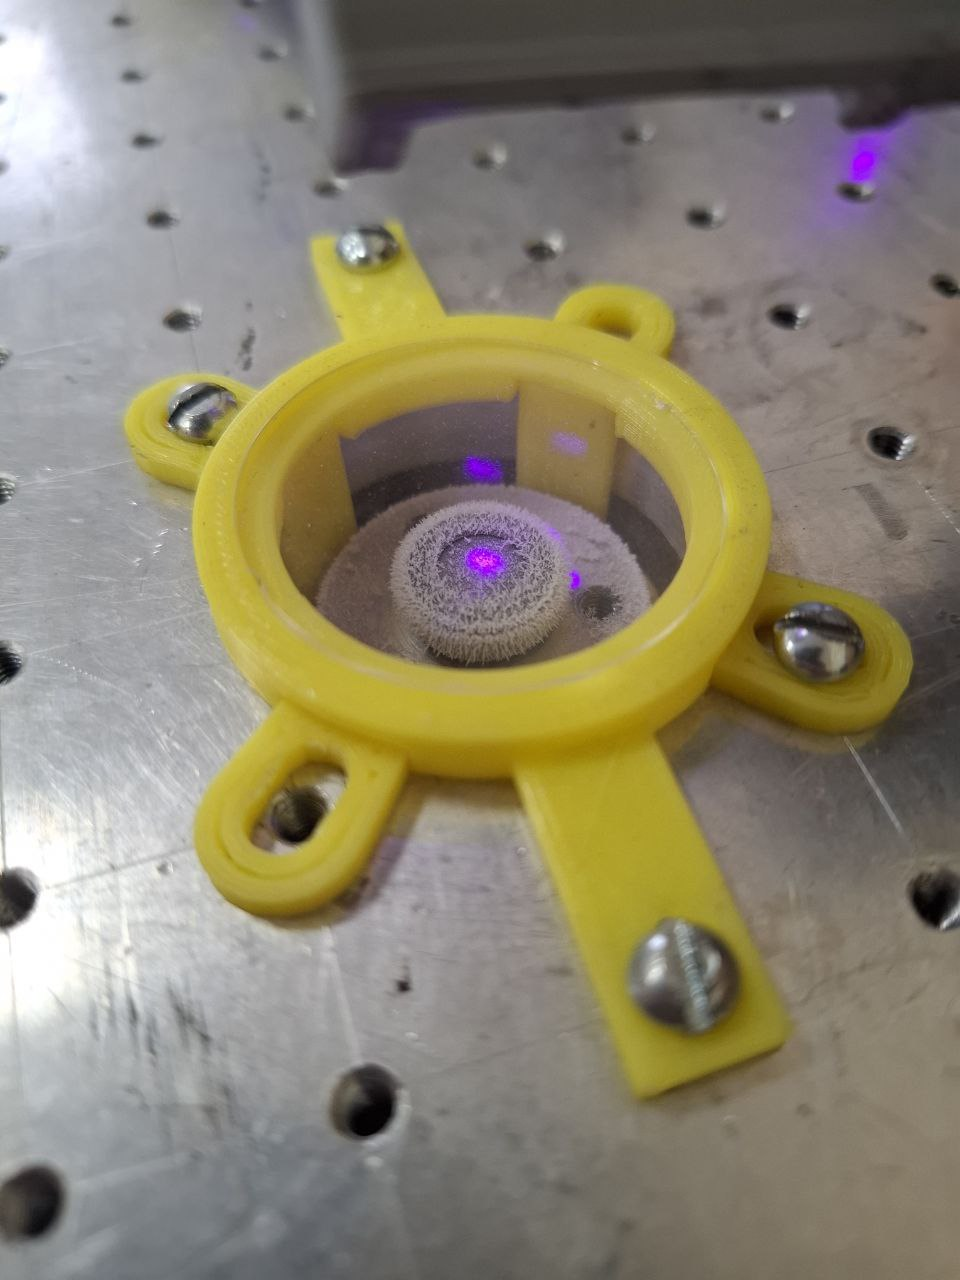
\includegraphics[width=0.5 \linewidth]{Beautiful.jpg}
        \caption{Замёрзший объектив}
        \label{Beautiful}
    \end{center}
\end{figure}